\chapter{Additional analysis results}
\label{app:analysis}

In this appendix we present results of the analysis that were left out of the body of the thesis. First we present the analysis of the effect of different window lengths $p$ ($1,5,10$ and $15$) on the detection performance in section \ref{sec:app_windowsizes}. In section \ref{sec:app_rp_standardized} we present the results corresponding to the analysis on the standardized data with the RP method and $\Delta$RP in comparison with baseline SPIRIT.

\section{Detection performance of RP with different window sizes}
\label{sec:app_windowsizes}
Throughout the body of this thesis we found that using a sliding window did not significantly improve the RP method nor the considered baseline SPIRIT. This is a logical observation for the RP method which does not take the temporal relations into account, but merely relies on the correlation among the different time series. For SPIRIT though, one might expect that it benefits from a sliding window. However, this specific method already incorporates a forgetting factor $\lambda$ that relates to the influence of the most recent part of the stream against its early history as explained in chapter \ref{chap:reconstruction-detection}. Still, the performance of SPIRIT is slightly affected by a sliding window since the forgetting factor is only a suboptimal solution to learn temporal relations to improve runtime performance. 

For the synthetic data set we used throughout the analysis, adding a sliding window mainly improves the detection performance of SPIRIT regarding the sensitivity to the number of projection vectors $k$. Logically, the runtime performance is much worse when we add a window. The effect of the number of projection vectors $k$ on the runtime is, however, very similar to what was already shown in figure \ref{fig:analysis_runtimes_point} in chapter \ref{chap:analysis}. Therefore, we do not present the runtime performances for different values of $p$.
Figure \ref{fig:app_aucs_point} shows the detection performances for global point outliers for the different window sizes. These results are presented and discussed in section \ref{sec:analysis_bird}, but were included for the sake of completeness.

\begin{figure}[h]
	\centering
	\includegraphics[scale=0.36]{analysis/AUCs_point}
	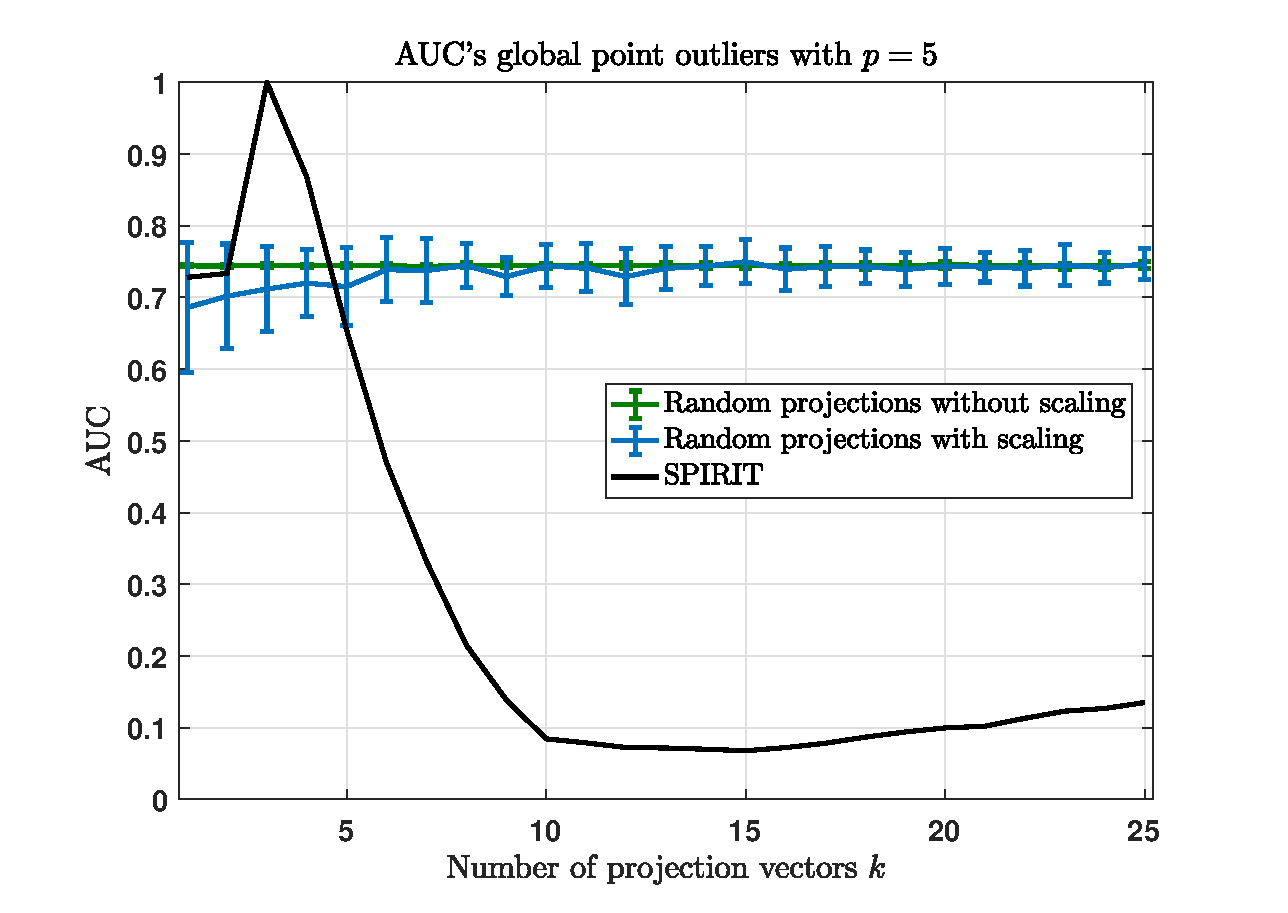
\includegraphics[scale=0.36]{analysis/AUCs_point1}
	\phantomcaption
	\label{fig:app_aucs_point}
\end{figure}%
\begin{figure}[h]\ContinuedFloat
	\centering
	\includegraphics[scale=0.36]{analysis/AUCs_point2}
	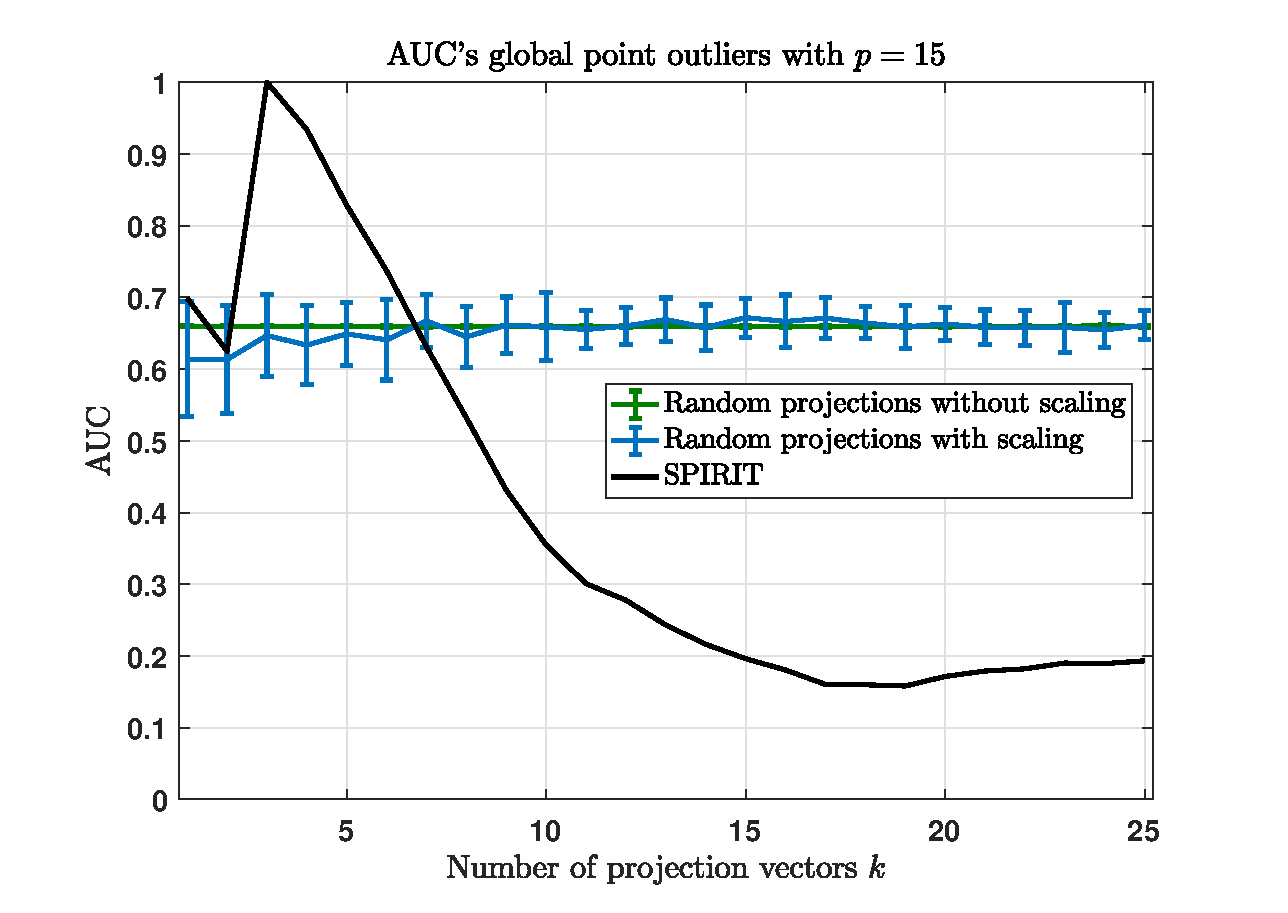
\includegraphics[scale=0.36]{analysis/AUCs_point3}
	\caption{Detection performances of global point outliers with $k$ from $1$ to $25$ for $p=\{1,5,10,15\}$.}
	\label{fig:app_aucs_point}
\end{figure}

\newpage
Figure \ref{fig:app_aucs_contextual} shows the performances corresponding to the detection of contextual point outliers. The only difference we observe here as a consequence of varying $p$ besides the poor performance in general, is that the AUC of the RP method improves a little when we adopt a sliding window.

\begin{figure}[h]
	\centering
	\includegraphics[scale=0.36]{analysis/AUCs_contextual}
	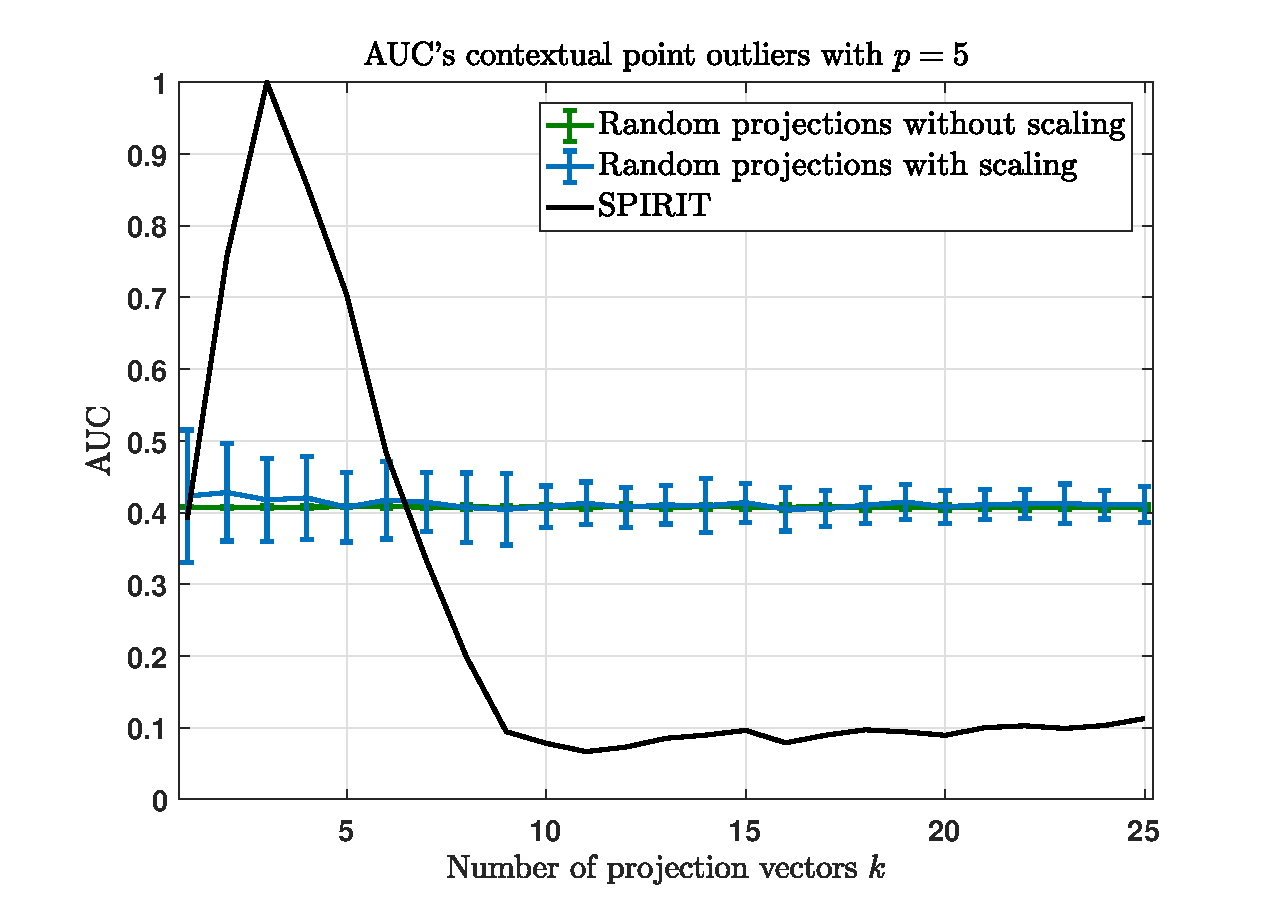
\includegraphics[scale=0.36]{analysis/AUCs_contextual1}
	\includegraphics[scale=0.36]{analysis/AUCs_contextual2}
	\includegraphics[scale=0.36]{analysis/AUCs_contextual3}
	\caption{Detection performances of contextual point outliers with $k$ from $1$ to $25$ for $p=\{1,5,10,15\}$.}
	\label{fig:app_aucs_contextual}
\end{figure}

Figure \ref{fig:app_aucs_collective} shows the performances corresponding to the detection of contextual collective outliers. Again, besides the poor performance, the main difference in behaviour is that the AUC of the RP method is slightly improved when adopting a sliding window.

\begin{figure}[h]
	\centering
	\includegraphics[scale=0.36]{analysis/AUCs_collective}
	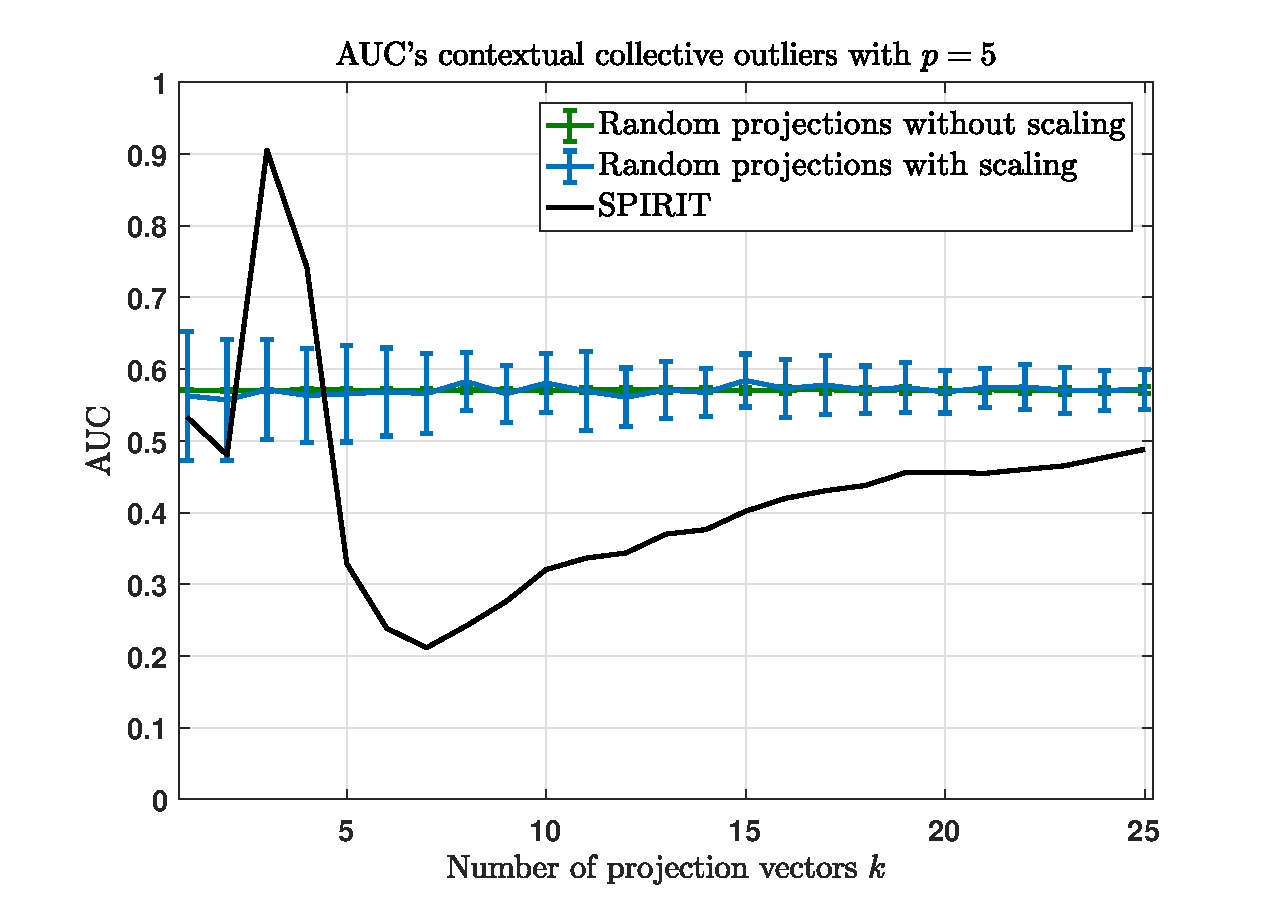
\includegraphics[scale=0.36]{analysis/AUCs_collective1}
	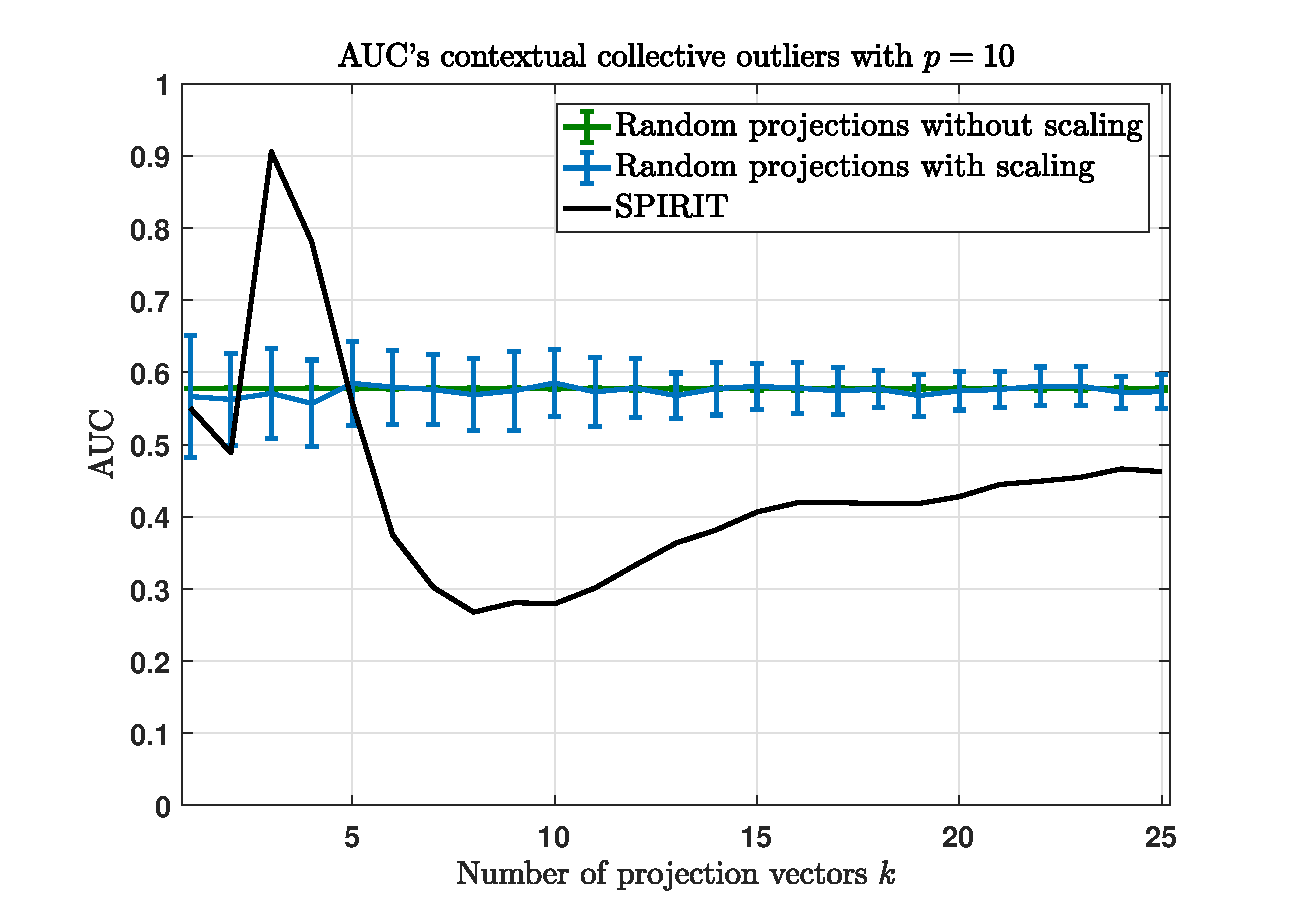
\includegraphics[scale=0.36]{analysis/AUCs_collective2}
	\includegraphics[scale=0.36]{analysis/AUCs_collective3}
	\caption{Detection performances of contextual collective outliers with $k$ from $1$ to $25$ for $p=\{1,5,10,15\}$.}
	\label{fig:app_aucs_collective}
\end{figure}

\newpage
\section{RP and \texorpdfstring{$\Delta$RP}{deltaRP} on standardized data}
\label{sec:app_rp_standardized}
In this section we present the results of the RP method in comparison to SPIRIT for the (offline) standardized versions of the synthetic data sets used in chapter \ref{chap:analysis}. We standardized the data set $\mathbf{X}$ by subtracting the mean of each $j^{\text{th}}$ time series ($\mu_j$) from each time series value $\mathbf{x}_{i,j}$ and divide the result by its standard deviation ($\sigma_j$) as in equation \eqref{eq:app_analysis_normalization}.

\begin{equation}\label{eq:app_analysis_normalization}
	\tilde{\mathbf{x}}_j = \frac{\mathbf{x}_j - \mu_j}{\sigma_j}
\end{equation}

As the behavioural observations of the performances with different window sizes are not significantly different from unstandardized data, we only present the results of the methods without a sliding window (i.e. $p=1$). The runtime of the RP-based methods is completely insensitive to the mean and range of the data, where the runtime of SPIRIT is also not affected significantly. Therefore, we did not include the runtime performances associated with the standardized data sets. 

Starting with the bird's-eye view of the RP method for standardized data, figure \ref{fig:app_aucs_standardized} shows the results for the number of projection vectors $k$ ranging from $1$ to $25$. 

\vspace{-0.25cm}
\hspace{-0.15cm}
\begin{figure}[h]
	\hspace{-0.2cm}
	\begin{minipage}{0.333\textwidth}
		\centering
		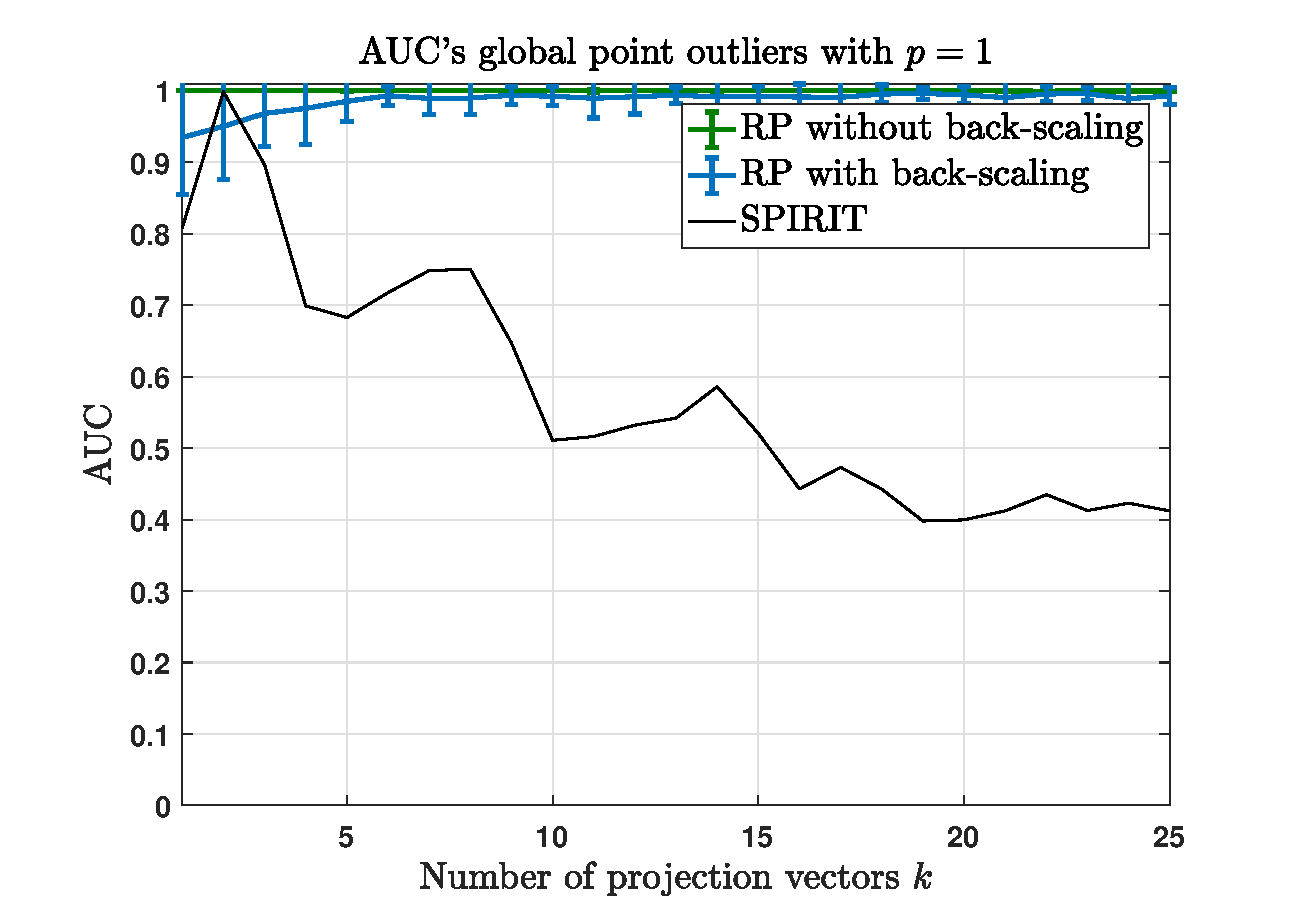
\includegraphics[scale=0.26]{analysis/AUCs_point_standardized}
	\end{minipage}
	\begin{minipage}{0.333\textwidth}
		\centering
		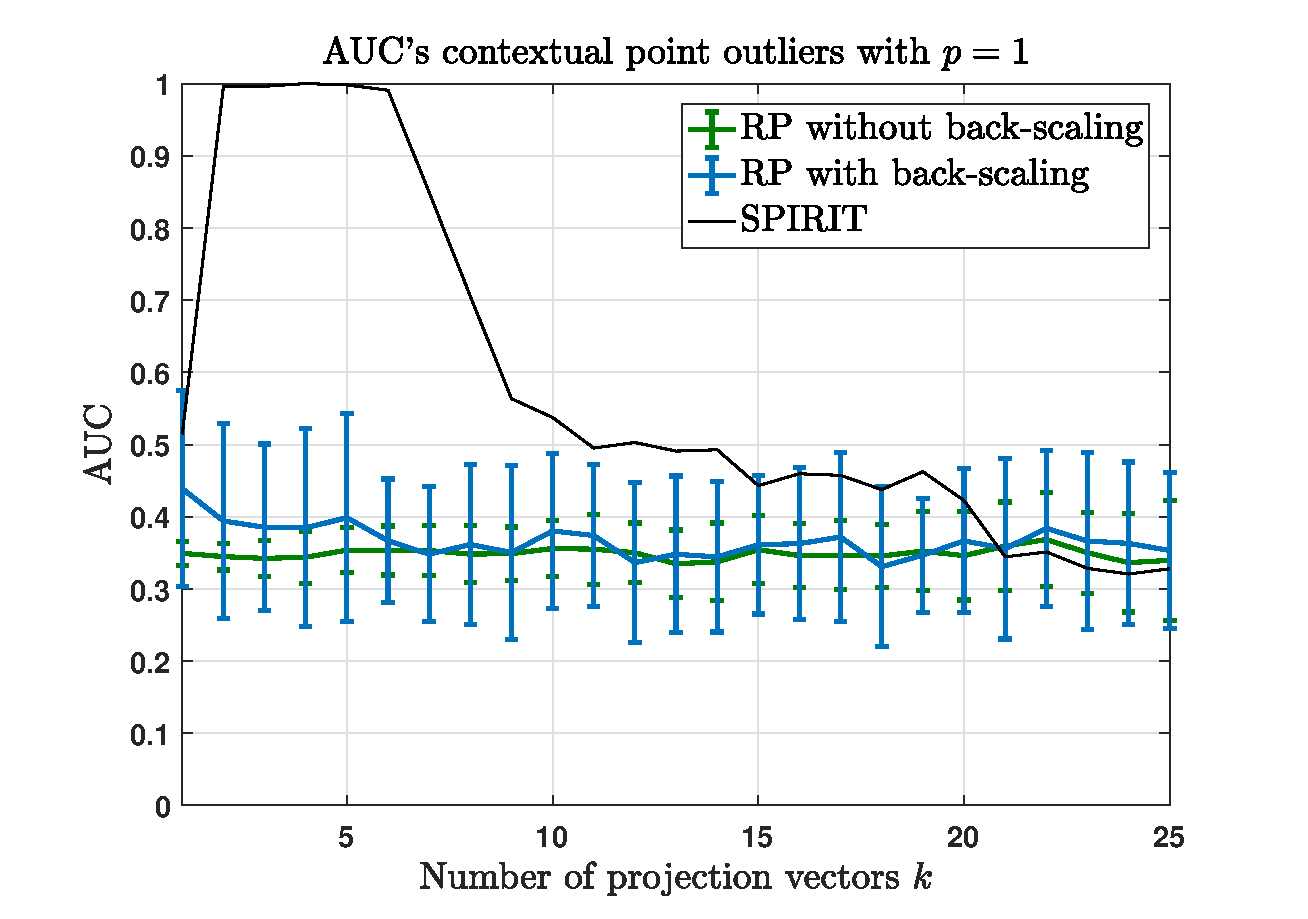
\includegraphics[scale=0.26]{analysis/AUCs_contextual_standardized}
	\end{minipage}
	\begin{minipage}{0.333\textwidth}
		\centering
		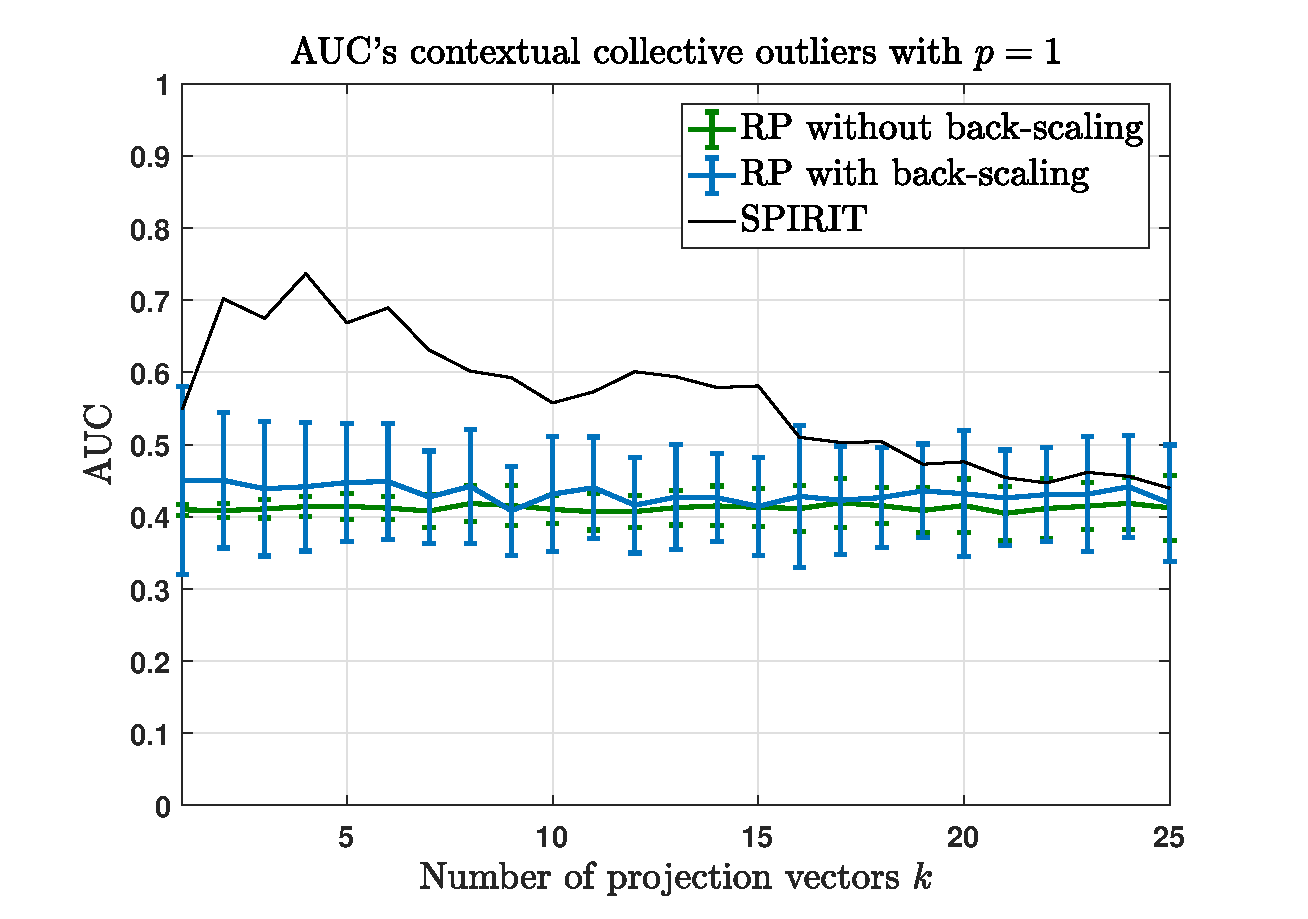
\includegraphics[scale=0.26]{analysis/AUCs_collective_standardized}
	\end{minipage}
	\caption{Detection performances of all three outlier types, with standardized data with $k$ from $1$ to $25$ for $p=1$.}
	\label{fig:app_aucs_standardized}
	\vspace{-0.2cm}
\end{figure}

For global point outliers (figure \ref{fig:app_aucs_standardized}, left), SPIRIT already reached an AUC of $1$ on unstandardized data and therefore no significant overall improvement can be detected. However, SPIRIT now has $3$ parameter settings ($k=1,2,3$) such that the AUC is above $0.80$. For the RP method we can clearly see that the performance is much better when the data is standardized as the RP method without back-scaling attains an AUC of $1$ irrespective of the number of projection vectors $k$, where its version with back-scaling approaches $1$ as well for sufficient $k$. Indeed, we can conclude that the RP method is not sensitive to $k$ in order to find global point outliers.

For contextual point outliers (figure \ref{fig:app_aucs_standardized}, center), especially SPIRIT improves regarding the AUC which now is close to $1$ for a larger range of the number of projection vectors $k$. That said, the RP method does not benefit from standardized data for finding contextual point outliers. A remarkable difference in the detection performances can be derived with respect to the contextual collective outliers (figure \ref{fig:app_aucs_standardized}, right). The RP method and baseline SPIRIT both perform worse for finding contextual collective outliers. While the RP methods (with and without back-scaling) obtained stable AUC's around $0.6$ and SPIRIT (at most) $0.9$, both optimal performances drop to $0.45$ and $0.73$, respectively.\\

Figure \ref{fig:app_aucs_spiritdelta_standardized} shows the detection performances of $\Delta$RP for different numbers of predictors $m$ in comparison with SPIRIT with different values for $k$. 

\hspace{-0.15cm}
\vspace{-0.2cm}
\begin{figure}[h]
	\hspace{-0.2cm}
	\begin{minipage}{0.333\textwidth}
		\centering
		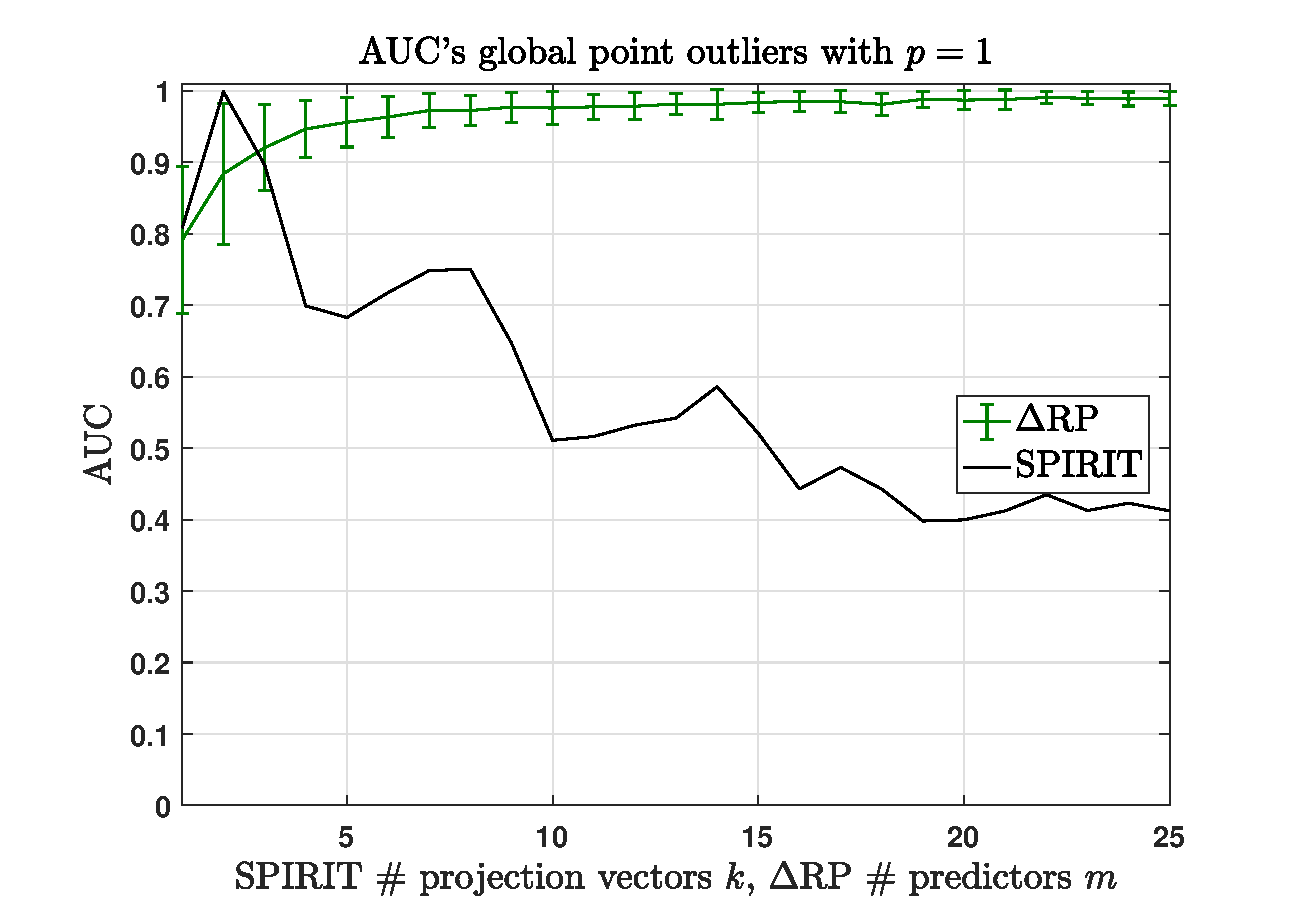
\includegraphics[scale=0.26]{analysis/AUCs_point_spiritdelta_standardized}
	\end{minipage}
	\begin{minipage}{0.333\textwidth}
		\centering
		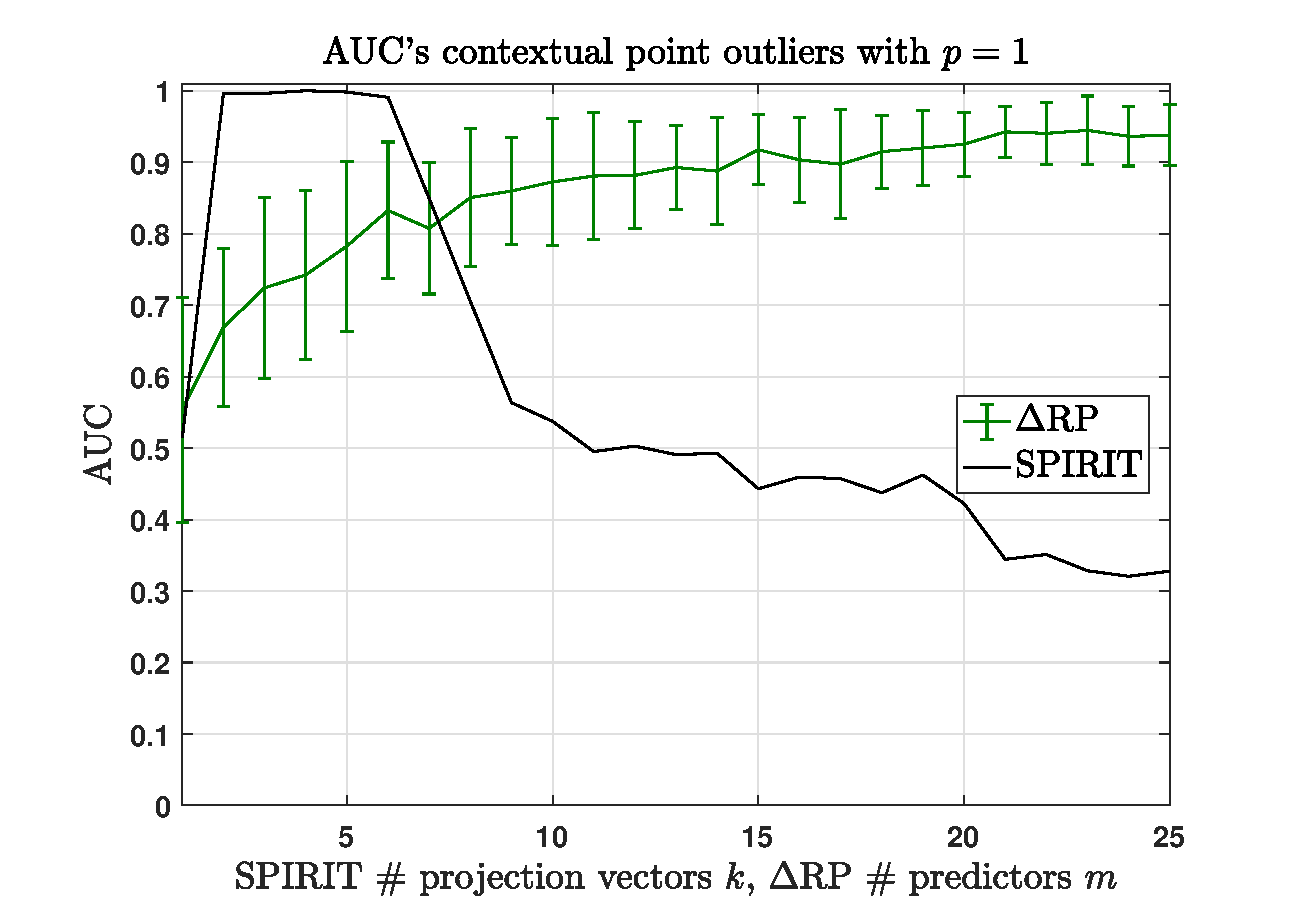
\includegraphics[scale=0.26]{analysis/AUCs_contextual_spiritdelta_standardized}
	\end{minipage}
	\begin{minipage}{0.333\textwidth}
		\centering
		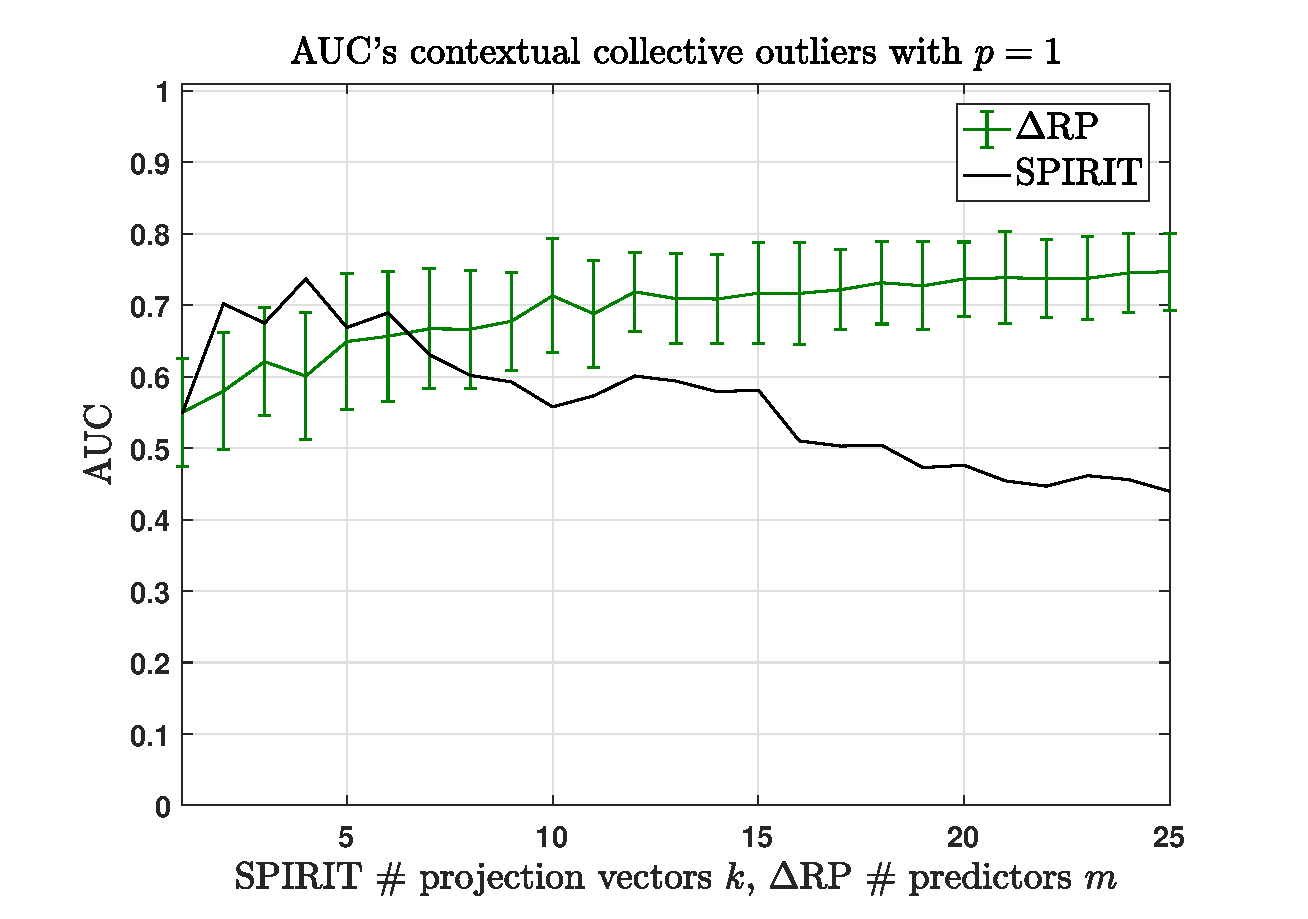
\includegraphics[scale=0.26]{analysis/AUCs_collective_spiritdelta_standardized}
	\end{minipage}
	\caption{Detection performances of all three outlier types, with standardized data with $k$ and $m$ from $1$ to $25$ for $p=1$.}
	\label{fig:app_aucs_spiritdelta_standardized}
	\vspace{0.1cm}
\end{figure}

Similar to the RP method, $\Delta$RP finds global point outliers (left) very accurately, approaching an AUC of $1$. In contrast to the RP method, however, it also successfully detects most contextual point outliers as well (center). Besides, it reaches an acceptable AUC with slightly less predictors than when the data is not standardized. For example, to obtain an AUC of approximately $0.90$ $\Delta$RP requires around $15$ predictors ($m=15$) when the data is not standardized. If standardization is possible, it attains an AUC of $0.90$ with around $12$ predictors ($m=12$). When it comes to the detection performance regarding contextual collective outliers (right), a similar observation can be made as for the RP method and SPIRIT. That is, finding contextual collective outliers apparently is harder when the data is standardized.

We also present the results of the methods when they are deployed in online mode on the standardized data. We used the same parameter settings as in table \ref{tab:analysis_parameters} which are presented again in table \ref{tab:app_analysis_parameters}. 

\begin{table}[h]
	\centering
	\vspace{0.05cm}
	\caption{Parameter settings for the analysis in online mode.}
	\label{tab:app_analysis_parameters}
	\begin{tabular}{l c c}
		\toprule
		\textbf{Method}					& \textbf{Parameter}		& \textbf{Value}		\\
		\midrule
		\multirow{2}{*}{SPIRIT} & $\lambda$				&$	0.97	$	\\
		& $[f_{\hat{E}}, F_{\hat{E}}]$	&	$[0.95, 0.98]$ \\
		\midrule
		RP				& $k$						&	$1$			\\
		$\Delta$RP		& $m$						&	$5$			\\
		\bottomrule		
	\end{tabular}
	\vspace{0.1cm}
\end{table}

In table \ref{tab:app_analysis_results_standrp} we present the results of the methods when deployed with these settings on the standardized data. For the sake of easy comparison, we also provide the results on the unstandardized data in table \ref{tab:app_analysis_results} as already presented in chapter \ref{chap:analysis}. All results were averaged over $50$ runs with distinct random projection matrices. Results that are significantly better than the opponent(s) according to the \textit{t}-statistic are made bold. 

\begin{table}[h]
	\centering
	\vspace{0.1cm}
	\caption{Online performances under fixed parameters on standardized data.}
	\label{tab:app_analysis_results_standrp}
	\small
	\begin{tabular}{l c c c c c c}
		\toprule	
		\multirow{3}{*}{\textbf{Method}}				&  \multicolumn{2}{c}{\textbf{Global point}}	& \multicolumn{2}{c}{\textbf{Contextual point}} & \multicolumn{2}{c}{\textbf{Contextual collective}}\\	
		\cmidrule{2-7}
		& 	AUC 	& Runtime 	& AUC 	& Runtime 	& AUC 	& Runtime 	\\
		\midrule
		SPIRIT	& $0.67	 $	&$	0.23 (\pm 0.07)	$&$	\mathbf{0.99 }$	& $	0.19 (\pm 0.06)$	& 	$\mathbf{0.65}$	& $0.22	(\pm 0.06)$ \\
		
		RP  	& $\mathbf{1.00	(\pm 0.00)}$	& $\mathbf{0.01 (\pm 0.01)}$ & $0.35 (\pm 0.01)$	& $\mathbf{0.01 (\pm 0.00)}$	& 	$	0.41 (\pm 0.01)$	& $\mathbf{0.01	(\pm 0.00)}$ \\
		
		$\Delta$RP		& $0.95 (\pm 0.04)$	&	$0.20 (\pm 0.1)$	&	$0.78 (\pm 0.11)$	& 	$0.20 (\pm 0.03)$	&	$\mathbf{0.64 (\pm 0.1)}$		&  $0.22 (\pm 0.07)$ \\
		\bottomrule
	\end{tabular}
	\vspace{0.1cm}
\end{table}

\begin{table}[h]
	\centering
	\caption{Online performances under fixed parameters on unstandardized data.}
	\label{tab:app_analysis_results}
	\small
	\hspace*{-0.25cm}
	\begin{tabular}{l c c c c c c}
		\toprule	
		\multirow{3}{*}{\textbf{Method}}				&  \multicolumn{2}{c}{\textbf{Global point}}	& \multicolumn{2}{c}{\textbf{Contextual point}} & \multicolumn{2}{c}{\textbf{Contextual collective}}\\	
		\cmidrule{2-7}
		& 	AUC 	& Runtime 	& AUC 	& Runtime 	& AUC 	& Runtime 	\\
		\midrule
		SPIRIT	& $0.79	 $	&$	0.30 (\pm 0.1)	$&$	0.55 $	& $	0.28 (\pm 0.07)$	& 	$	0.58$	& $0.25	(\pm 0.06)$ \\
		
		RP  	& $0.90	(\pm 0.01)$	& $\mathbf{0.01 (\pm 0.00)}$ & $0.28 (\pm 0.01)$	& $\mathbf{0.02 (\pm 0.01)}$	& 	$	0.57 (\pm 0.01)$	& $\mathbf{0.02	(\pm 0.01)}$ \\
		
		$\Delta$RP		& $\mathbf{0.95 (\pm 0.05)}$	&	$0.21 (\pm 0.06)$	&	$\mathbf{0.71 (\pm 0.16)}$	& 	$0.21 (\pm 0.07)$	&	$\mathbf{0.71 (\pm 0.09)}$		&  $0.22 (\pm 0.04)$	\\
		\bottomrule
	\end{tabular}
	\vspace{0.1cm}
\end{table}

%\newpage
In contrast to SPIRIT, RP perfectly finds the global point outliers as a consequence of the power of the squared Euclidean distance \cite{zimek2012survey}. Yet its performance with regard to the contextual outlier types is not competitive with SPIRIT and $\Delta$RP. The latter for that matter is competitive with the best performing method for global point (RP) and contextual collective outliers (SPIRIT), yet not close to the AUC of $0.99$ obtained with SPIRIT for finding contextual point outliers. 

SPIRIT finds the contextual point outliers very well as its AUC is $0.99$ compared to an AUC of $0.55$ for the unstandardized data. This complies with the observation from figures \ref{fig:app_aucs_standardized} and \ref{fig:app_aucs_spiritdelta_standardized} that SPIRIT is less sensitive to the value for the number of projection vectors $k$ when the data is standardized. That is, it obtains an AUC around $1$ for $k$ ranging from $2$ to $6$ instead of for only one value for $k$ as the case with unstandardized data. 

Concerning the runtime performances, the RP method evidently outperforms $\Delta$RP and SPIRIT. In contrast to the experiments with unstandardized data, there is no significant difference between SPIRIT and $\Delta$RP, which shows that the runtime of SPIRIT depends on the mean and range of the data as well.
That SPIRIT is sensitive to the mean and range of the data can also be concluded from the larger differences between the performances on unstandardized and standardized data compared to the RP method and $\Delta$RP. This holds for the runtime as well detection performance.

The ROC curves in figure \ref{fig:analysis_rocs_point_scaled} show the balance between the TPR and FPR corresponding to the presented AUC's in table \ref{tab:app_analysis_results_standrp}. It becomes more clear how $\Delta$RP is much more stable considering the detection performance. That is, it yields a reasonable to good performance irrespective of the outlier type, where the default RP method still only finds global outliers and SPIRIT is only significantly (much) better in finding contextual point outliers.

\begin{figure}[h]
	\begin{minipage}{0.333\textwidth}
		\centering
		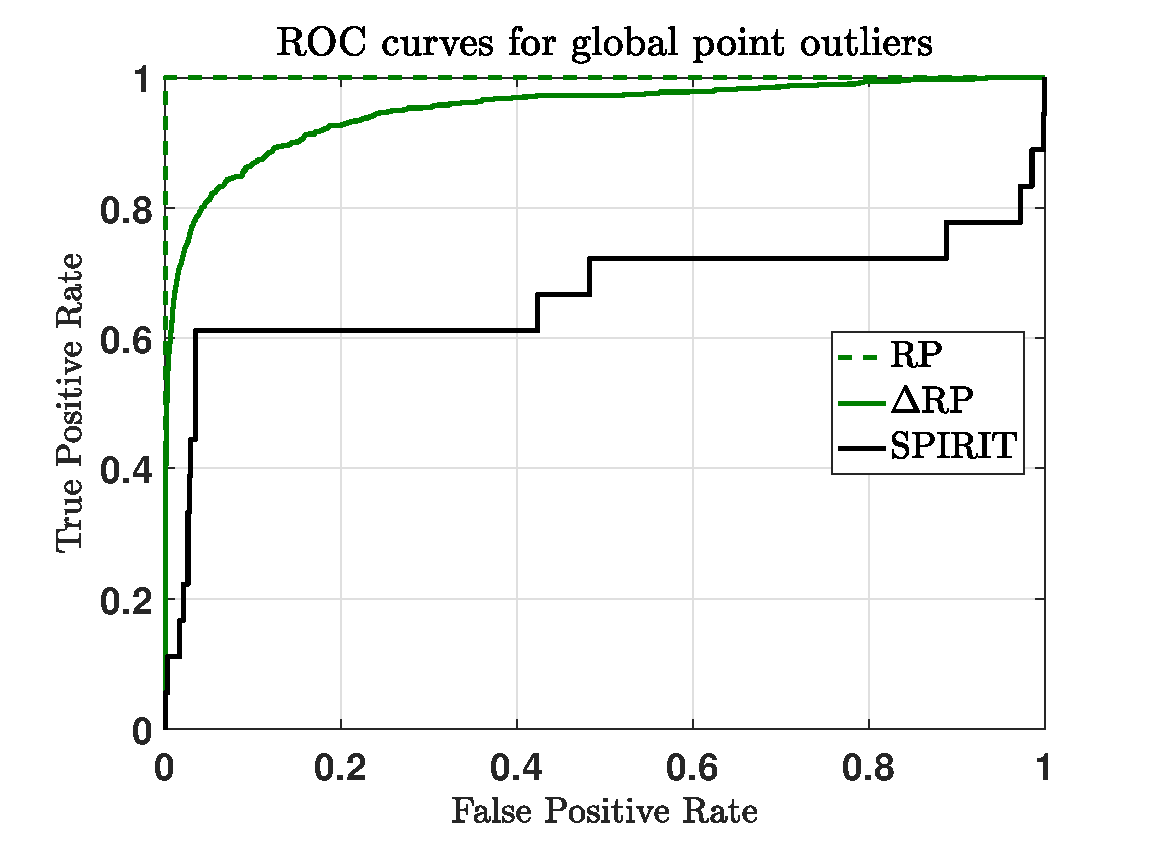
\includegraphics[scale=0.28]{analysis/ROCs_point_scaled}
	\end{minipage}
	\begin{minipage}{0.333\textwidth}
		\centering
		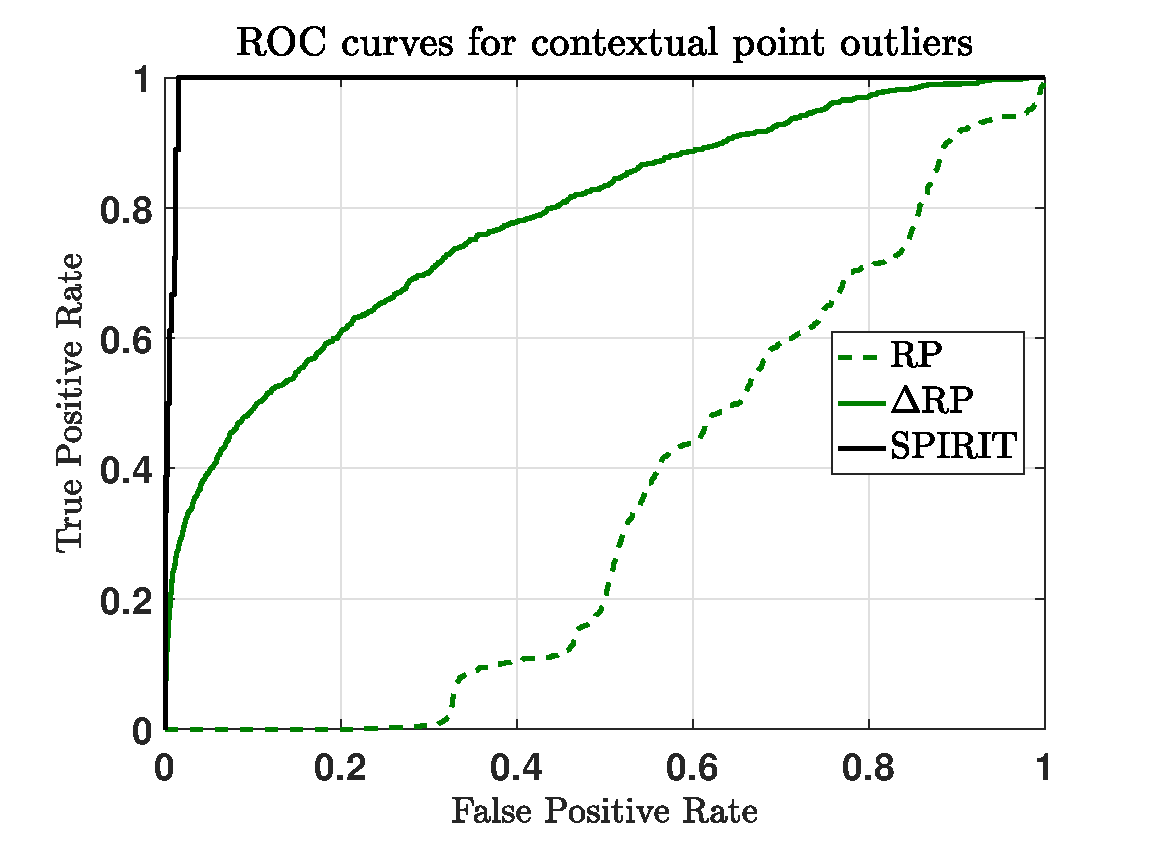
\includegraphics[scale=0.28]{analysis/ROCs_contextual_scaled}
	\end{minipage}
	\begin{minipage}{0.333\textwidth}
		\centering
		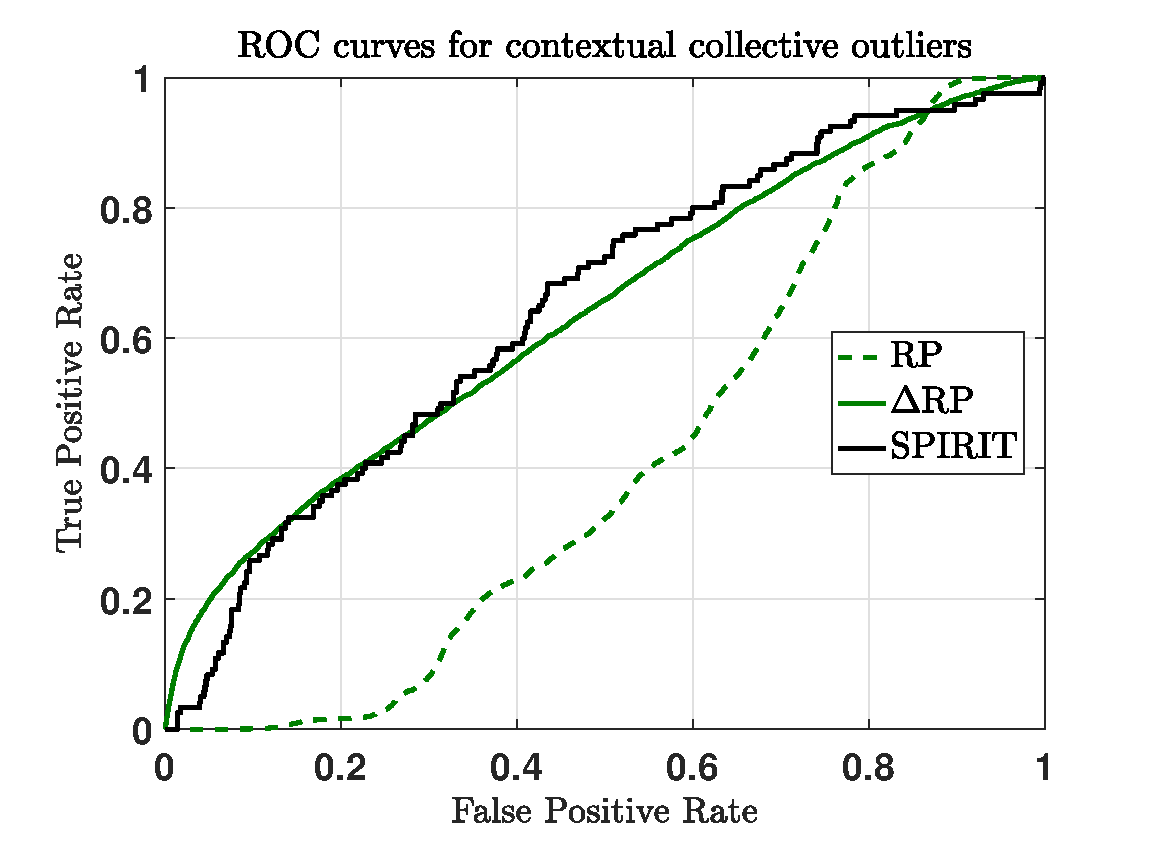
\includegraphics[scale=0.28]{analysis/ROCs_collective_scaled}
	\end{minipage}
	\caption{ROC curves of RP, $\Delta$RP and SPIRIT for the three general outlier types in the standardized data.}
	\label{fig:analysis_rocs_point_scaled}
\end{figure}



